\documentclass[8pt,aspectratio=169]{beamer}
\usetheme{Madrid}
\usepackage{graphicx,booktabs,adjustbox,multicol,amsmath,amssymb,listings,xcolor,colortbl}
\definecolor{mlblue}{RGB}{0,102,204}
\definecolor{mlpurple}{RGB}{51,51,178}
\definecolor{mllavender}{RGB}{173,173,224}
\definecolor{mllavender2}{RGB}{193,193,232}
\definecolor{mllavender3}{RGB}{204,204,235}
\definecolor{mllavender4}{RGB}{214,214,239}
\definecolor{mlorange}{RGB}{255,127,14}
\definecolor{mlgreen}{RGB}{44,160,44}
\definecolor{mlred}{RGB}{214,39,40}
\definecolor{mlgray}{RGB}{127,127,127}
\definecolor{termgreen}{RGB}{0,200,0}
\definecolor{termbg}{RGB}{30,30,30}
\setbeamercolor{palette primary}{bg=mllavender3,fg=mlpurple}
\setbeamercolor{palette secondary}{bg=mllavender2,fg=mlpurple}
\setbeamercolor{palette tertiary}{bg=mllavender,fg=white}
\setbeamercolor{palette quaternary}{bg=mlpurple,fg=white}
\setbeamercolor{structure}{fg=mlpurple}
\setbeamercolor{title}{fg=mlpurple}
\setbeamercolor{frametitle}{fg=mlpurple,bg=mllavender3}
\setbeamercolor{block title}{bg=mllavender2,fg=mlpurple}
\setbeamercolor{block body}{bg=mllavender4,fg=black}
\setbeamertemplate{navigation symbols}{}
\setbeamertemplate{itemize items}[circle]
\setbeamersize{text margin left=5mm,text margin right=5mm}
\newcommand{\bottomnote}[1]{\vfill\vspace{-2mm}\textcolor{mllavender2}{\rule{\textwidth}{0.4pt}}\par\vspace{1mm}{\footnotesize\textbf{\adjustbox{max width=\textwidth}{#1}}}}
\usepackage{tikz}
\usetikzlibrary{arrows.meta,positioning,shapes.geometric,calc,chains,decorations.pathmorphing,automata,fit}
\usepackage{pgfplots}
\pgfplotsset{compat=1.18}
\title{Deploy a Token from Python --- Colab Notebook Walkthrough}
\author{Prof.~Dr.~Joerg Osterrieder}
\institute{University Lecture Series}
\date{\today}
\begin{document}

%% ============================================================
%% FRAME 1: TITLE PAGE
%% ============================================================
\begin{frame}[plain]
\vspace{2cm}
\begin{center}
{\Large\bfseries\color{mlpurple} Deploy a Token from Python}\\[4mm]
{\large\color{mlblue} Colab Notebook Walkthrough}\\[8mm]
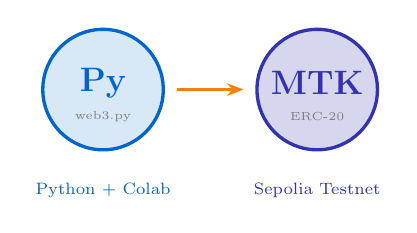
\begin{tikzpicture}[scale=0.85, every node/.style={transform shape}]
% Python logo (simplified)
\draw[mlblue, very thick, fill=mlblue!15] (-1.2,0) circle (0.9);
\node[font=\Large\bfseries, mlblue] at (-1.2,0.1) {Py};
\node[font=\tiny, mlgray] at (-1.2,-0.4) {web3.py};
% Arrow
\draw[-{Stealth[length=6pt]}, mlorange, very thick] (-0.1,0) -- (0.9,0);
% Ethereum icon
\draw[mlpurple, very thick, fill=mllavender4] (2.0,0) circle (0.9);
\node[font=\Large\bfseries, mlpurple] at (2.0,0.1) {MTK};
\node[font=\tiny, mlgray] at (2.0,-0.4) {ERC-20};
% Labels
\node[font=\scriptsize, mlblue] at (-1.2,-1.5) {Python + Colab};
\node[font=\scriptsize, mlpurple] at (2.0,-1.5) {Sepolia Testnet};
\end{tikzpicture}
\\[6mm]
{\footnotesize Prof.~Dr.~Joerg Osterrieder}\\[1mm]
{\footnotesize\color{mlgray} University Lecture Series}
\end{center}
\bottomnote{No Remix, no Hardhat --- just Python in a browser.}
\end{frame}

%% ============================================================
%% FRAME 2: THE PYTHON TOOLCHAIN
%% ============================================================
\begin{frame}{The Python Toolchain}
\begin{center}
\adjustbox{max width=\textwidth}{%
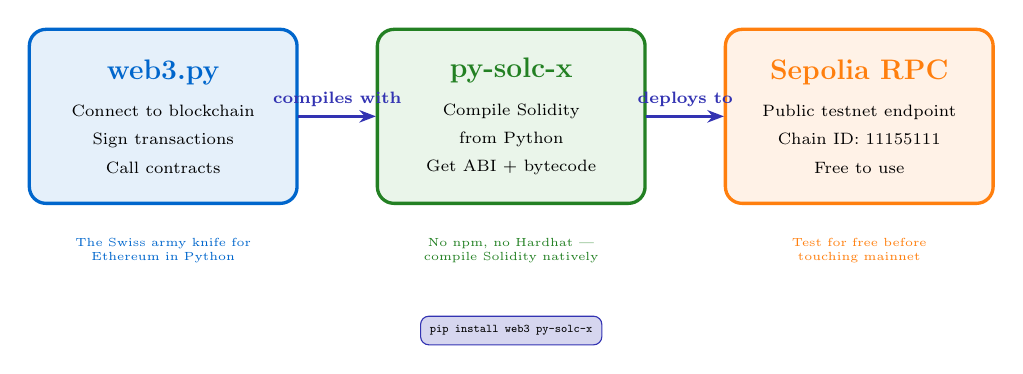
\begin{tikzpicture}[scale=0.85, every node/.style={transform shape},
  toolbase/.style={very thick, rounded corners=6pt,
    minimum height=2.6cm, minimum width=4.0cm, align=center}]

% Box 1: web3.py
\node[toolbase, draw=mlblue, fill=mlblue!10] (web3) at (-5.2,0) {%
  \textbf{\large\color{mlblue}web3.py}\\[4pt]
  \scriptsize Connect to blockchain\\
  \scriptsize Sign transactions\\
  \scriptsize Call contracts};

% Box 2: py-solc-x
\node[toolbase, draw=mlgreen!80!black, fill=mlgreen!10] (solc) at (0,0) {%
  \textbf{\large\color{mlgreen!80!black}py-solc-x}\\[4pt]
  \scriptsize Compile Solidity\\
  \scriptsize from Python\\
  \scriptsize Get ABI + bytecode};

% Box 3: Sepolia RPC
\node[toolbase, draw=mlorange, fill=mlorange!10] (rpc) at (5.2,0) {%
  \textbf{\large\color{mlorange}Sepolia RPC}\\[4pt]
  \scriptsize Public testnet endpoint\\
  \scriptsize Chain ID: 11155111\\
  \scriptsize Free to use};

% Arrows
\draw[-{Stealth[length=6pt]}, mlpurple, very thick] (web3.east) -- (solc.west)
  node[midway, above, font=\scriptsize\bfseries] {compiles with};
\draw[-{Stealth[length=6pt]}, mlpurple, very thick] (solc.east) -- (rpc.west)
  node[midway, above, font=\scriptsize\bfseries] {deploys to};

% Descriptions below
\node[font=\tiny, mlblue, text width=3.8cm, align=center] at (-5.2,-2.0)
  {The Swiss army knife for\\Ethereum in Python};
\node[font=\tiny, mlgreen!80!black, text width=3.8cm, align=center] at (0,-2.0)
  {No npm, no Hardhat ---\\compile Solidity natively};
\node[font=\tiny, mlorange, text width=3.8cm, align=center] at (5.2,-2.0)
  {Test for free before\\touching mainnet};

% pip install annotation
\node[draw=mlpurple, fill=mllavender4, rounded corners=3pt, font=\tiny\ttfamily,
      inner sep=4pt] at (0,-3.2) {pip install web3 py-solc-x};

\end{tikzpicture}%
}%
\end{center}
\bottomnote{Two pip packages and a public RPC URL --- that is the entire toolchain.}
\end{frame}

%% ============================================================
%% FRAME 3: THE DEPLOYMENT PIPELINE
%% ============================================================
\begin{frame}{The Deployment Pipeline}
\vspace{-2mm}
\begin{columns}[T]
\begin{column}{0.48\linewidth}
\adjustbox{max width=\linewidth}{%
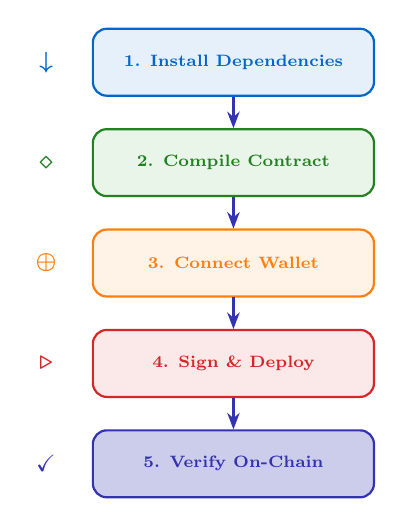
\begin{tikzpicture}[scale=0.85, every node/.style={transform shape},
  stepbox/.style={draw=mlpurple, thick, fill=mllavender4, rounded corners=5pt,
    minimum height=1.0cm, minimum width=4.2cm, align=center, font=\scriptsize\bfseries},
  icon/.style={font=\normalsize, mlpurple}]

% Step 1
\node[stepbox, draw=mlblue, fill=mlblue!10] (s1) at (0,5.5)
  {\color{mlblue}1. Install Dependencies};
\node[icon, mlblue] at (-2.8,5.5) {$\boldsymbol{\downarrow}$};

% Step 2
\node[stepbox, draw=mlgreen!80!black, fill=mlgreen!10] (s2) at (0,4.0)
  {\color{mlgreen!80!black}2. Compile Contract};
\node[icon, mlgreen!80!black] at (-2.8,4.0) {$\boldsymbol{\diamond}$};

% Step 3
\node[stepbox, draw=mlorange, fill=mlorange!10] (s3) at (0,2.5)
  {\color{mlorange}3. Connect Wallet};
\node[icon, mlorange] at (-2.8,2.5) {$\boldsymbol{\oplus}$};

% Step 4
\node[stepbox, draw=mlred, fill=mlred!10] (s4) at (0,1.0)
  {\color{mlred}4. Sign \& Deploy};
\node[icon, mlred] at (-2.8,1.0) {$\boldsymbol{\triangleright}$};

% Step 5
\node[stepbox, draw=mlpurple, fill=mllavender3] (s5) at (0,-0.5)
  {\color{mlpurple}5. Verify On-Chain};
\node[icon] at (-2.8,-0.5) {$\checkmark$};

% Arrows
\draw[-{Stealth[length=6pt]}, mlpurple, thick] (s1.south) -- (s2.north);
\draw[-{Stealth[length=6pt]}, mlpurple, thick] (s2.south) -- (s3.north);
\draw[-{Stealth[length=6pt]}, mlpurple, thick] (s3.south) -- (s4.north);
\draw[-{Stealth[length=6pt]}, mlpurple, thick] (s4.south) -- (s5.north);

\end{tikzpicture}%
}%
\end{column}
\begin{column}{0.50\linewidth}
\adjustbox{max width=\linewidth, max totalheight=6.2cm}{%
\scriptsize
\renewcommand{\arraystretch}{1.25}
\begin{tabular}{@{}>{\bfseries\color{mlpurple}}l p{2.6cm} p{2.4cm}@{}}
\toprule
\textbf{\color{mlpurple}Step} & \textbf{\color{mlblue}Python Code} & \textbf{\color{mlgreen!80!black}On-Chain Effect} \\
\midrule
\rowcolor{mlblue!6}
1 & {\tiny\texttt{pip install web3 py-solc-x}} & None (local setup) \\
2 & {\tiny\texttt{solcx.compile\_source()}} & None (local compile) \\
\rowcolor{mlblue!6}
3 & {\tiny\texttt{Web3(HTTPProvider())}} & RPC handshake \\
4 & {\tiny\texttt{sign\_transaction()}} & Tx broadcast, contract created \\
\rowcolor{mlblue!6}
5 & {\tiny\texttt{token.functions.name()}} & Read-only call \\
\bottomrule
\end{tabular}%
}%
\end{column}
\end{columns}
\bottomnote{Five cells in Colab, five steps from zero to a live token --- the notebook mirrors this pipeline exactly.}
\end{frame}

%% ============================================================
%% FRAME 4: WHAT THE NOTEBOOK OUTPUTS
%% ============================================================
\begin{frame}{What the Notebook Outputs}
\begin{center}
\adjustbox{max width=\textwidth, max totalheight=6.5cm}{%
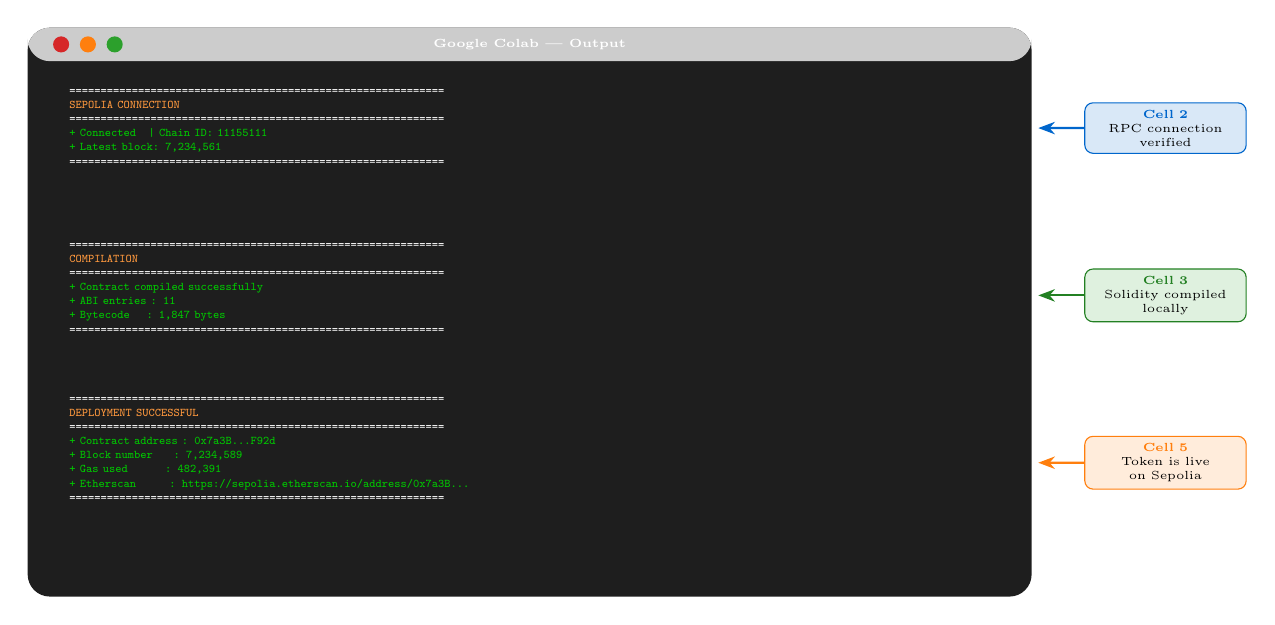
\begin{tikzpicture}[scale=0.85, every node/.style={transform shape}]

% Terminal background
\fill[termbg, rounded corners=8pt] (-7.5,-4.5) rectangle (7.5,4.0);
% Title bar
\fill[mlgray!40, rounded corners=8pt] (-7.5,3.5) rectangle (7.5,4.0);
\node[font=\tiny\bfseries, white] at (0,3.75) {Google Colab --- Output};
% Dots
\fill[mlred] (-7.0,3.75) circle (0.12);
\fill[mlorange] (-6.6,3.75) circle (0.12);
\fill[mlgreen] (-6.2,3.75) circle (0.12);

% Block 1: CONNECTION
\node[font=\tiny\ttfamily, termgreen, anchor=north west, text width=14cm, align=left]
  at (-7.0,3.2) {%
\textcolor{white}{============================================================}\\
\textcolor{mlorange!80!white}{SEPOLIA CONNECTION}\\
\textcolor{white}{============================================================}\\
\textcolor{termgreen}{+ Connected~~~| Chain ID: 11155111}\\
\textcolor{termgreen}{+ Latest block: 7,234,561}\\
\textcolor{white}{============================================================}};

% Block 2: COMPILATION
\node[font=\tiny\ttfamily, termgreen, anchor=north west, text width=14cm, align=left]
  at (-7.0,0.9) {%
\textcolor{white}{============================================================}\\
\textcolor{mlorange!80!white}{COMPILATION}\\
\textcolor{white}{============================================================}\\
\textcolor{termgreen}{+ Contract compiled successfully}\\
\textcolor{termgreen}{+ ABI entries : 11}\\
\textcolor{termgreen}{+ Bytecode~~~~: 1,847 bytes}\\
\textcolor{white}{============================================================}};

% Block 3: DEPLOYMENT
\node[font=\tiny\ttfamily, termgreen, anchor=north west, text width=14cm, align=left]
  at (-7.0,-1.4) {%
\textcolor{white}{============================================================}\\
\textcolor{mlorange!80!white}{DEPLOYMENT SUCCESSFUL}\\
\textcolor{white}{============================================================}\\
\textcolor{termgreen}{+ Contract address : 0x7a3B...F92d}\\
\textcolor{termgreen}{+ Block number~~~~~: 7,234,589}\\
\textcolor{termgreen}{+ Gas used~~~~~~~~~: 482,391}\\
\textcolor{termgreen}{+ Etherscan~~~~~~~~: https://sepolia.etherscan.io/address/0x7a3B...}\\
\textcolor{white}{============================================================}};

% Annotations on the right
\node[draw=mlblue, fill=mlblue!15, rounded corners=3pt, font=\tiny,
      inner sep=3pt, text width=2.2cm, align=center]
      (a1) at (9.5,2.5) {\textbf{\color{mlblue}Cell 2}\\RPC connection\\verified};
\draw[-{Stealth[length=6pt]}, mlblue, thick] (a1.west) -- (7.6,2.5);

\node[draw=mlgreen!80!black, fill=mlgreen!15, rounded corners=3pt, font=\tiny,
      inner sep=3pt, text width=2.2cm, align=center]
      (a2) at (9.5,0.0) {\textbf{\color{mlgreen!80!black}Cell 3}\\Solidity compiled\\locally};
\draw[-{Stealth[length=6pt]}, mlgreen!80!black, thick] (a2.west) -- (7.6,0.0);

\node[draw=mlorange, fill=mlorange!15, rounded corners=3pt, font=\tiny,
      inner sep=3pt, text width=2.2cm, align=center]
      (a3) at (9.5,-2.5) {\textbf{\color{mlorange}Cell 5}\\Token is live\\on Sepolia};
\draw[-{Stealth[length=6pt]}, mlorange, thick] (a3.west) -- (7.6,-2.5);

\end{tikzpicture}%
}%
\end{center}
\bottomnote{Three output blocks confirm success --- connection, compilation, and deployment with an Etherscan link.}
\end{frame}

%% ============================================================
%% FRAME 5: KEY TAKEAWAYS
%% ============================================================
\begin{frame}{Key Takeaways}
\vspace{-2mm}
\begin{center}
\adjustbox{max width=\textwidth,max totalheight=6.8cm}{%
\scriptsize
\renewcommand{\arraystretch}{1.4}
\begin{tabular}{@{}c >{\raggedright\arraybackslash}p{10.5cm}@{}}
\toprule
\textbf{\color{mlpurple}\#} & \textbf{\color{mlpurple}Takeaway} \\
\midrule
\rowcolor{mlpurple!6}
\textbf{\Large\color{mlpurple}1} & \textbf{Python can deploy smart contracts} --- no Remix needed. A Colab notebook with \texttt{web3.py} replaces the entire browser-based IDE workflow. \\
\textbf{\Large\color{mlblue}2} & \textbf{py-solc-x compiles Solidity locally} --- no npm, no Hardhat, no Node.js. One \texttt{pip install} gives you a full Solidity compiler in Python. \\
\rowcolor{mlpurple!6}
\textbf{\Large\color{mlgreen!70!black}3} & \textbf{web3.py signs and sends transactions} --- your private key never leaves your machine. The key is read with \texttt{getpass} and used only to sign locally. \\
\textbf{\Large\color{mlorange}4} & \textbf{Sepolia testnet is free} --- experiment without risk. Test ETH comes from public faucets and the RPC endpoint is open to everyone. \\
\rowcolor{mlpurple!6}
\textbf{\Large\color{mlred}5} & \textbf{The same code works for mainnet} --- just change the RPC URL and chain ID. Everything else (compile, sign, deploy) stays identical. \\
\bottomrule
\end{tabular}
}%
\end{center}
\bottomnote{Five cells, two pip packages, zero cost --- Python is the fastest path from idea to deployed token.}
\end{frame}

\end{document}
